\documentclass{report}
\usepackage{tkz-euclide}
\usepackage{tikz}
\usepackage{textpos}
\usepackage{tikz}
\usepackage{tikz-3dplot}
\usepackage{tkz-euclide}
\usepackage{chemfig}

\begin{document}
	\begin{figure}
\begin{scriptsize}
		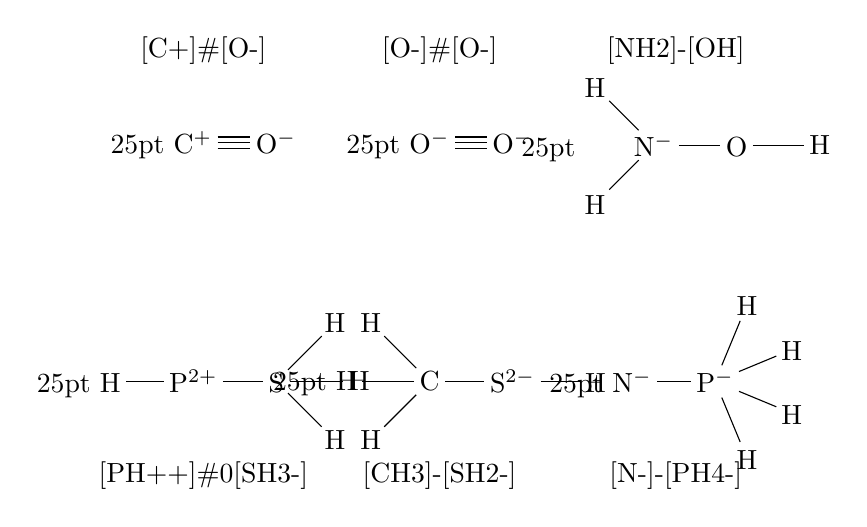
\begin{tikzpicture}
%		\draw[thick, use as bounding box](-1,-1) rectangle (10,5);
		% % % %
		
		\node [color=black] (lab11) at (1,4.7) {[C+]\#[O-]};
		
		\node (met) at (1,3.5){\setatomsep{25pt}
		\chemfig{C^+(~[:0]O^{-})}};
		
		% % %
		\node [color=black] (lab21) at (4,4.7) {[O-]\#[O-]};
		\node (met21) at (4,3.5){
			\setatomsep{25pt}
			\chemfig{O^{-}(~[:0]O^{-})}};
		
		
		% % %
		\node [color=black] (lab12) at (1,-0.7) {[PH++]\#0[SH3-]};
		
		\node (met12) at (1,0.5){\setatomsep{25pt}
		\chemfig{P^{2+}(-[:0]S(-[:45]H)(-[:0]H)(-[:315]H))(-[:180]H)}};
		
		
		% % %
		\node [color=black] (lab12) at (4,-0.7) {[CH3]-[SH2-]};
		
		\node (met) at (4,0.5){\setatomsep{25pt}
		\chemfig{C(-[:0]S^{2{-}}(-[:0]H))(-[:135]H)(-[:180]H)(-[:225]H)}};
		
		
		% % %
		\node [color=black] (lab12) at (7,4.7) {[NH2]-[OH]};
		\node (met) at (7,3.5){\setatomsep{25pt}
		\chemfig{N^{-}(-[:0]O-H)(-[:135]H)(-[:225]H)}};
		
		
		% % %
		\node [color=black] (lab12) at (7,-0.7) {[N-]-[PH4-]};
		
		\node (met) at (7,0.5){\setatomsep{25pt}
		\chemfig{N^{-}(-[:0]P^{-}(-[:22.5]H)(-[:67.5]H)(-[:292.5]H)(-[:337.5]H))}};
		\end{tikzpicture}
	\end{scriptsize}
	\centering
	\caption{First heavy atom is the connecting atom.}
	\end{figure}

\end{document}